\subsubsection{Contrastive Hebbian Learning}

\paragraph{My notes.}
%TODO citations 
%TODO rewrite 
%TODO shorten 
%TODO write it as a comparison to BAL and GeneRec, i.e. put it into context 

The point of this article \citet{movellan1990contrastive} is that a convenient learning rule is derived from a standard Hopfield energy function. Then Movellan uses insights of annealing to improve the training phase and avoid the learning function to settle in local minima. These improvements are formalized in the next five rules applied sequentially:

To assess the effect of interactivity, two different networks were compared on the combinatorial generaliza-
tion task, a standard feedforward backpropagation network, and an interactive GeneRec network using the
symmetric, midpoint variation learning rule which is equivalent to contrastive Hebbian learning (CHL) or a
deterministic Boltzmann machine (DBM) \citet{o1996bio}, \citet{o2001generalization}. 

\begin{enumerate}
\item Activation are reset to random numbers after each learning phase. 

\item First settle for the clamped phase (+), and then, without resetting activations, free the output units and settle again. 

\item Settle during the free pase and then, without resetting activations, clamp the output units and resettle again. 

\item Sharpening Schedules (annealing Peterson and Hartman 1989)

\item Annealing schedules: In search of the continuous Boltzmann machine. This may be achieved in interactive networks by injecting some form of noise to the net input of each unit. The standard deviation of the noise distribution plays a similar effect to the temperature parameter in descrete Boltzmann machines \citet{movellan1990contrastive}. 
\end{enumerate}

Movellan introduced notation for the plus (+) phase when both input and output are clamped and minus (-) phase when input is clamped and output is free. 

%TODO: How the activations are changed? 
%TODO: Are the activation of CHL same as in GeneRec (so just the update rule is changed?) 
%TODO prekreslit do IPE 
\begin{center} 
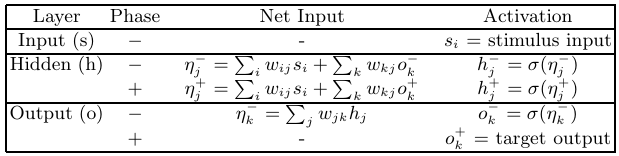
\includegraphics{img/table_generec.png} 
\citet{farkas2013bal} 
\end{center} 

\paragraph{Original equations.}
Define a continuous Hopfield Energy function $F = E + S$ where
$$ E = -\frac{1}{2}\sum_i\sum_ja_iw_{ij}a_j$$
and 
$$ S = \sum_i \int_{rest}^{a_i} f_i^{-1}(a)da.$$
and $a^T = [a_1,\ldots,a_n]$ is the activation vector, $f_i$ is bounded, monotically increasing, differentiable activation function \citet{movellan1990contrastive}.

\paragraph{Simplified model.}

$$\frac{1}{\epsilon}\Delta w_{ij} = (a_i^+a_j^+)-(a_i^-a_j^-),$$
where $a_i$ is the seind unit and $a_j$ is the receiving unit. 

Decreasing the energy
$$E = \sum_j\sum_i a_j a_i w_{ij}.$$

\paragraph{O'Reillys conclusion.}

The two phases of activation states used in CHL are the plus phase states, which result from both input
and target being presented to the network, and provide a training signal when compared to the minus phase
activations, which result from just the input pattern being presented \citet{o1996bio}. 

